% Decentralized multispectral UAV swarm for search and rescue.
% Build:  cd paper && tectonic swarm_sar_paper.tex      (or pdflatex twice)
% All numbers come from results/README.md (1,620 paired simulated missions).
\documentclass[conference]{IEEEtran}
\IEEEoverridecommandlockouts

\usepackage[nocompress]{cite}
\usepackage{amsmath,amssymb}
\usepackage{fontspec}
\renewcommand{\dbltopfraction}{0.95}\renewcommand{\dblfloatpagefraction}{0.7}\setcounter{dbltopnumber}{4}\renewcommand{\topfraction}{0.9}\setcounter{topnumber}{3}
% Times-compatible text font with real bold and italic shapes (XeTeX cannot embolden the default Type 1 Times)
\IfFontExistsTF{TeX Gyre Termes}{\setmainfont{TeX Gyre Termes}}{\IfFontExistsTF{Nimbus Roman}{\setmainfont{Nimbus Roman}}{}}
\usepackage{graphicx}
\usepackage{dblfloatfix}
\usepackage{booktabs}
\usepackage{xcolor}
\usepackage{url}
\usepackage{algorithm}
\usepackage{algorithmic}
\usepackage{tikz}
\usetikzlibrary{positioning,arrows.meta,fit,backgrounds,calc}
\usepackage[colorlinks=true,linkcolor=blue!60!black,citecolor=blue!60!black,urlcolor=blue!60!black,breaklinks=true]{hyperref}
\graphicspath{{../results/figures/}{./figures/}{./}}

\newcommand{\cli}[1]{\texttt{-{}-#1}}
\newcommand{\pmsd}[2]{#1{\scriptsize$\pm$#2}}

\setlength{\textfloatsep}{6pt plus 2pt minus 2pt}\setlength{\floatsep}{6pt plus 2pt minus 2pt}\setlength{\intextsep}{6pt plus 2pt minus 2pt}
\begin{document}

\title{Decentralized Multispectral UAV Swarms for Search and Rescue: Early-Fusion Perception, Delay-Tolerant Networking, and Energy-Aware Self-Organization}

\author{\IEEEauthorblockN{Devesh Agarwal, Naman Chaudhary, Sankalp Mittal}
\IEEEauthorblockA{\textit{Under the Guidance of Dr. Rayanoothala Praneetha Sree} \\
\textit{Department of Information Technology} \\
\textit{National Institute of Technology Raipur} \\
Chhattisgarh - 492010, India}
}

\maketitle

\begin{abstract}
Searching a large disaster area with a UAV swarm requires reliable person detection in poor light, continued operation after the loss of an aircraft, and delivery of findings over radio links that are mostly unavailable. Existing coordination and routing methods usually assume a connected network or a central planner. This paper presents a decentralized search-and-rescue system for such conditions that integrates three components: a 4-channel RGB and thermal early-fusion YOLO11 detector, a delay-tolerant mesh with store-carry-forward alert relaying, and a coordination layer that combines energy-weighted centroidal Voronoi tessellation (EW-CVT), dual-threshold hysteresis, sector claiming and lease-based failure detection. Every UAV plans from its own, possibly outdated, view of the swarm. We evaluate the system in a kinematic simulator that uses real multispectral frames, over 1{,}620 paired missions with confidence intervals. Buffering raises the share of victims known to the operator from 3.4\% to 98\% in a 5\,km arena, and failover recovers 11 points of coverage after a UAV is lost. Epidemic relaying delivers alerts 7.6\,s sooner than spray-and-wait at 3\,km, but it keeps about two more copies of each alert. After a loss, the survivors need about 230\,s to detect it, because no UAV can know of the loss before the missing one is overdue at base. All results come from simulation, and we discuss the limits of this evidence.
\end{abstract}

\begin{IEEEkeywords}
UAV swarm, search and rescue, multispectral fusion, delay-tolerant networking, decentralized coverage control, centroidal Voronoi tessellation
\end{IEEEkeywords}

%=====================================================================
\section{Introduction}
The first hours after an earthquake or a flood largely determine who is found alive, and the survival rate drops sharply with time \cite{speth2022}. Small unmanned aerial vehicles (UAVs) can cover a wide area much faster than ground teams, and a swarm can cover it faster still. However, several practical problems stand in the way of using a swarm in a real disaster. Visible-light cameras perform poorly in shadow or smoke, where a thermal camera can still show a person. Over areas several kilometres wide the swarm is mostly out of radio contact, so a design that assumes a connected network would deliver almost nothing. A single ground planner would be a single point of failure and would need links that disaster areas rarely offer, whereas UAVs that act on their own may duplicate or abandon work when batteries differ and a UAV is lost unnoticed.

We study perception, communication and control together, because what a UAV can decide depends on what it has heard, and what it hears depends on the radio link. The main contributions of this paper are as follows:
\begin{enumerate}
\item An integrated decentralized architecture for search and rescue with intermittently connected swarms, which combines a 4-channel RGB and thermal early-fusion detector (YOLO11) with delay-tolerant alert dissemination and energy-aware coordination.
\item A coordination layer that works on stale local views. It uses an energy-weighted partition (EW-CVT) with dual-threshold hysteresis, claim-and-yield sector assignment, and lease-based failure detection that treats silence as normal and releases work only at base.
\item A delay-tolerant alert mechanism with per-recipient buffers and store-carry-forward relaying, evaluated under a physical radio model.
\item A controlled evaluation over 1{,}620 paired simulated missions, with a component-wise ablation and a comparison with spray-and-wait, buffering only, a static partition and a nearest-bidder auction without failover. We report the effects with confidence intervals, including the unfavourable ones.
\end{enumerate}


%=====================================================================
\section{Related Work}\label{sec:related}
\textbf{UAVs for search and rescue.} Small UAVs have been used to support wilderness and disaster search since the field trials of Goodrich et al.\ \cite{goodrich2008}. For several robots, exploration and task allocation have been studied by Burgard et al.\ \cite{burgard2005} and by Gerkey and Matari\'c \cite{gerkey2004}, and auction-based methods decide which robot searches which part of the area. Grøntved et al.\ \cite{grontved2023} adapt such an auction to search and rescue and assume a fully connected network, and Giacomossi et al.\ \cite{giacomossi2026} re-auction the sectors of a failed UAV, but the failure is reported by the UAV itself and the simulation has no radio losses. These methods assume reliable communication or reach agreement by consensus \cite{olfatisaber2007}, whereas our setting resembles flying ad hoc networks with sparse, intermittent links \cite{bekmezci2013}.

\textbf{Multispectral person detection.} Combining visible and thermal images is known to improve pedestrian detection in poor light \cite{hwang2015kaist,jia2021llvip}. Early fusion, in which the two modalities are stacked as input channels, needs little extra computation and is therefore suitable for onboard hardware \cite{speth2022}. We use it on top of the YOLO family \cite{redmon2016yolo,jocher2024yolo11}. Speth et al.\ \cite{speth2022} released the multispectral dataset that we use, and our detector follows their early-fusion design.

\textbf{Coverage control.} Dividing an area among agents with Voronoi cells and moving each agent to the centroid of its cell (Lloyd iteration) is a standard coverage method \cite{lloyd1982,du1999cvt,cortes2004coverage}. In contrast, our agents act on outdated views received over a lossy link and resolve conflicts by claiming sectors. Weighting the distance by a quantity that belongs to each agent gives a weighted Voronoi diagram. A power diagram \cite{aurenhammer1987power} subtracts the weight from the squared distance, and we divide by it instead. Energy-aware versions of Lloyd's method use such weights to give smaller regions to robots with less energy \cite{kwok2007,munir2024}. Our weight represents the battery level in the same way, so we do not claim the weighting itself as new. The weight rule of Munir et al.\ \cite{munir2024} reduces to our case $\alpha=1$ when all UAVs drain at similar rates, so we do not run it separately. We add hysteresis to the updates to avoid chattering when the inputs are noisy.

\textbf{Failure detection.} Deciding that a peer has failed when the channel is unreliable is the problem addressed by unreliable failure detectors \cite{chandra1996}. Accrual detectors \cite{hayashibara2004} rely on heartbeat arrival times, which does not suit a mesh in which silence is normal. Instead, our sortie lease follows the lease idea of Gray and Cheriton \cite{gray1989}. A claim is valid until a stated time, and after that time it can be released.

\textbf{Delay-tolerant networking.} When end-to-end paths rarely exist, nodes can store messages and forward them when they meet other nodes \cite{fall2003dtn}. Epidemic and spray-and-wait routing \cite{vahdat2000epidemic,spyropoulos2005spray} trade the delivery rate against the number of copies and the buffer use. We use epidemic forwarding with a buffer cap, and Section~\ref{sec:base} compares it with spray-and-wait and buffering only in the same simulator. The simulator builds on FlyNetSim \cite{baidya2018flynetsim}, and our radio model is a simple log-distance channel \cite{rappaport2002wireless}. The per-recipient buffers follow DMLT \cite{kosaka2023dmlt}.

%=====================================================================
\section{Problem Formulation}\label{sec:problem}
A team of $N$ UAVs launches from a common base and searches an $L\times L$ arena divided into $K$ sectors with centres $c_s$. UAV $i$ has a position, a battery level $B_i\in[0,B_{\max}]$ and a set of claimed sectors. An unknown set of victims lies in the sectors, and a UAV that scans a sector raises an alert for each victim that it detects. The radio links are lossy and time-varying: the packet error rate between two UAVs depends on their distance (Eq.~\ref{eq:pl}), so the communication graph is mostly disconnected in flight. The ground control station (GCS) is a passive sink at the base.

The objective is to maximize the coverage of the arena and the share of victims whose alert reaches the GCS (the operator recall), while keeping the mission time and the alert latency short. Three constraints apply. A UAV must return to base before its battery falls below a 15\% reserve. There is no central planner, so every decision may use only the information that the UAV has itself received. A UAV may also be lost without notice.

%=====================================================================
\section{Proposed Methodology}\label{sec:method}
\subsection{System Architecture}
Fig.~\ref{fig:arch} gives an overview of the proposed system. Every UAV runs the same three components. \emph{Perception} turns a multispectral frame of the sector below into victim detections. \emph{Mesh communication} sends alerts and periodic status messages over a lossy radio link, buffers what could not be sent, and carries received alerts onward. \emph{Control} chooses which sectors to search, from the UAV's own battery and its current view of its peers, and builds a route. The ground control station (GCS) is a passive sink: it receives alerts and plans nothing.

The interfaces are narrow: alerts go from perception to the mesh, status messages update the control view of the peers, and control hands a route to flight. The aircraft and the radio are simulated, whereas the detection, networking and control logic is the code under test.

\begin{figure*}[!t]
\centering
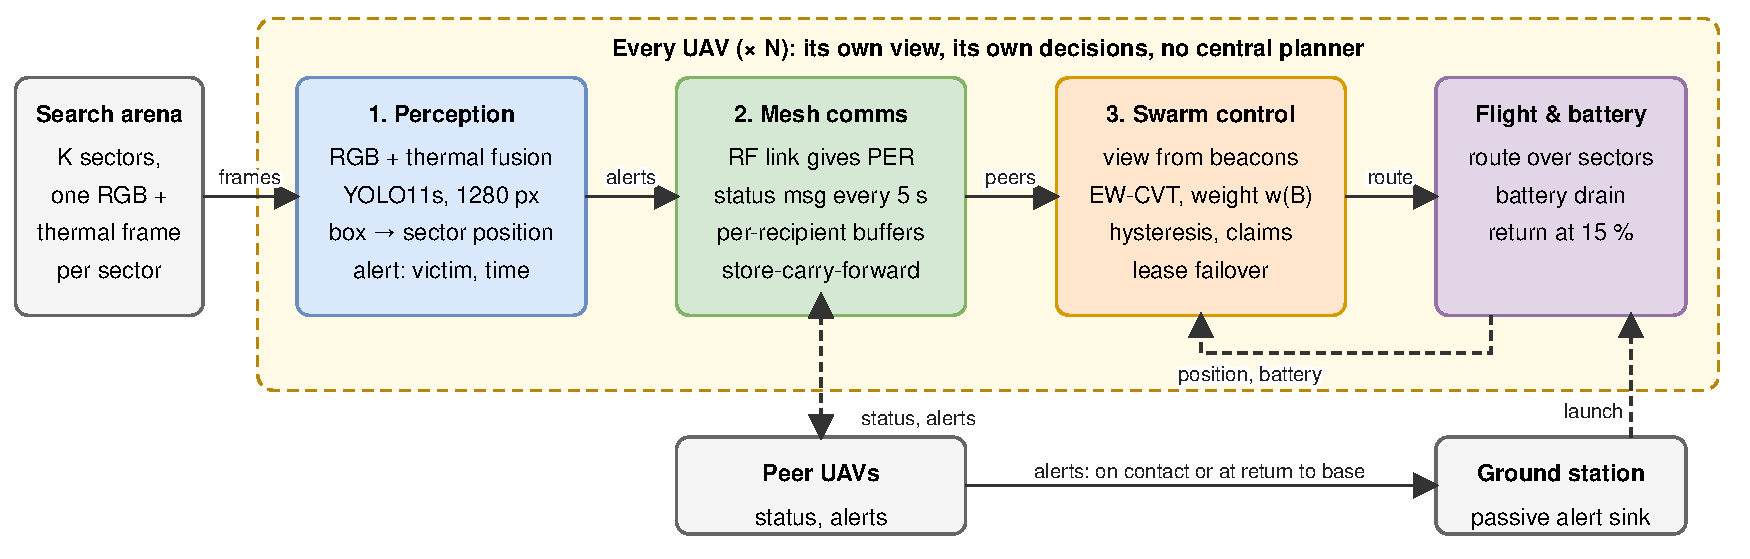
\includegraphics[width=0.84\textwidth]{architecture.pdf}
\caption{System architecture. Solid arrows: data flow; dashed arrows: feedback, radio exchange and launch.}
\label{fig:arch}
\end{figure*}

%=====================================================================
\subsection{Multispectral Victim Detection}
The visible (RGB) and thermal long-wave infrared frames are stacked into a four-plane tensor, and the first convolution of the detector takes four input channels. The shipped model is YOLO11s with an input size of 1280\,px, and the frames are $1280{\times}937$. It is trained on the NII-CU Multispectral Aerial Person Detection dataset \cite{speth2022}, with a single person class. We initialise the thermal kernel with the pretrained red-channel kernel, and we train without colour jitter because it has no meaning for a thermal plane. The box centre of a detection is mapped linearly into the bounds of the sector in which the frame was taken, which gives a world coordinate. This is sector-based georeferencing. It is not a camera model.

\subsection{Wireless Channel Model}
The path loss between two UAVs at distance $d$ is modelled by Eq.~\ref{eq:pl}.
\begin{equation}
PL(d)=PL(d_0)+10\,n\log_{10}\tfrac{d}{d_0}+X_\sigma+\Delta_{\text{obs}},
\label{eq:pl}
\end{equation}
where $\Delta_{\text{obs}}=15$\,dB when the link is obstructed (a random 10\% chance beyond 50\,m) and 0 otherwise,
with $PL(d_0)=20\log_{10}f_{\text{MHz}}-27.55$, $n=2.5$, $d_0=1$\,m, log-normal shadowing $X_\sigma$ with $\sigma=4$\,dB, and a noise floor of $-90$\,dBm. SNR $=P_{tx}-PL-N_0$ maps to a packet error rate: PER $=0$ above 25\,dB, $1$ below 5\,dB, and $1-(1+e^{-0.5(\text{SNR}-15)})^{-1}$ between. Arenas of 2\,km or more use 33\,dBm at 2.4\,GHz, giving PER $\approx0.5$ at about 520\,m; smaller arenas use 30\,dBm at 5\,GHz (about 220\,m). Against arenas of several kilometres, the swarm is mostly disconnected in flight.

\subsection{Delay-Tolerant Alert Dissemination}
\emph{a) Alert generation and buffering.} When a UAV detects a victim, it makes one direct attempt to reach every other UAV and the GCS. Each failed copy is stored in a per-recipient QoS-1 buffer. The buffer is flushed when the link to that recipient has a PER below 0.2, which in practice happens when the UAV returns to base.

\emph{b) Store-carry-forward relaying.} This is epidemic forwarding \cite{vahdat2000epidemic}: a UAV that \emph{receives} an alert also keeps a copy for each recipient that is not known to hold it, and it hands the copy over when it later meets that recipient with a good link. No UAV needs to be in the right place at the right moment, and an alert survives the loss of its finder. On contact, only the copies that the other side lacks are sent, and a full buffer drops its oldest copy.

\emph{c) Status messages.} Every 5\,s, each UAV broadcasts its position, its committed EW-CVT generator and weight, its state, the time at which its route should bring it home, its sector claims, and the set of sectors that it knows to be scanned. These messages are single-hop and are not buffered, since stale state is not worth delivering late. A receiver merges the scanned sets as grow-only sets, and thus the knowledge about coverage spreads transitively when UAVs meet.

\subsection{Energy-Weighted Territory Partitioning}
Let $B_i$ be the battery level of UAV $i$ and $B_{\max}$ the capacity. The UAV has the weight $w_i=(B_i/B_{\max})^{\alpha}$. A sector with centre $c_s$ is preferred by the UAV with the smallest weighted distance
\begin{equation}
d(s,i)=\frac{\lVert c_s-g_i\rVert^2}{\max(0.01,\,w_i)},
\label{eq:pd}
\end{equation}
where $g_i$ is the committed generator of the UAV. For $\alpha=0$ the partition is a plain Voronoi diagram, and a larger $\alpha$ shrinks the territory of low-battery UAVs. The launch partition is the converged CVT (15 Lloyd iterations).

\subsection{Decentralized Coordination and Failure Detection}
Algorithm~\ref{alg:tick} summarizes one control tick of a UAV, and its steps are described below.
\emph{a) Dual-threshold hysteresis.} Every 5\,s, each UAV computes the centroid $C_i^*$ that its cell should have. It does so over the peers that it \emph{believes} to be active, using their last advertised generators and weights. The UAV commits the new generator and weight only if
\begin{equation}
U_i=\big(\Delta B_i\ge\tau_\epsilon\ \wedge\ \lVert C_i^*-C_i\rVert\ge\tau_\delta\big)\ \vee\ \big(\mathcal N_i(t)\ne\mathcal N_i(t_k)\big),
\label{eq:commit}
\end{equation}
with $\tau_\epsilon=2\%$ of $B_{\max}$, $\tau_\delta=5$\,m, and $\mathcal N_i$ the view of the live set held by the UAV. Without this gate, noisy battery readings would commit a new partition at every tick.

\emph{b) Claim-and-yield sector assignment.} A UAV claims a sector if it is the preferred owner by $d(s,i)$ (Eq.~\ref{eq:pd}) using committed values and no other UAV holds a valid claim on the sector. It keeps its existing claims unless a better claim (a smaller $d$, with ties broken by id) reaches it. It may take over the claim of a peer only if it would arrive well before the advertised arrival time of that peer. A UAV that has no claims left takes the nearest unclaimed sector. Routes are greedy nearest-neighbour tours that end at the launch pad.

\emph{c) Lease-based failure detection.} In flight, silence tells a UAV nothing about a peer, because the peer may be out of range or it may have landed. Instead, each peer advertises the time at which its route should bring it home. A peer that is still missing \textit{slack} seconds after this time (60\,s by default) is suspected to be lost, and its claims are released. Since a lost peer looks like one that landed quietly, released work is taken only by UAVs \emph{at base}, which have heard the landed peers. Landed UAVs listen for 10\,s, split the work among themselves by $d(s,i)$, and relaunch if the battery allows. A suspicion is withdrawn when the peer is heard again. A UAV aborts and returns at 15\% battery, and it is lost at 0\%.

\begin{algorithm}[t]
\caption{Control tick of one UAV (every 5\,s).}\label{alg:tick}
\footnotesize
\begin{algorithmic}[1]
\STATE merge any status messages received since the last tick into the view (peers, claims, scanned set)
\STATE \textbf{for} each peer $j$ overdue at base by more than \textit{slack}: mark $j$ suspected; release its claims
\STATE $\mathcal N_i\leftarrow$ self $\cup$ peers believed active (landed peers included only if self is at base)
\STATE read own battery $B_i$; $w_i^*\leftarrow(B_i/B_{\max})^{\alpha}$; $C_i^*\leftarrow$ EW-CVT centroid of my cell over $\mathcal N_i$
\STATE \textbf{if} $U_i$ (Eq.~\ref{eq:commit}) \textbf{then} commit $g_i\leftarrow C_i^*$, $w_i\leftarrow w_i^*$
\STATE keep claims not beaten by a better claim; add free sectors I prefer by $d(s,i)$
\STATE \textbf{if} no claims left: claim nearest unclaimed sector; \textbf{if} at base: also share released work
\STATE \textbf{if} claims changed: rebuild route; advertise route ETA, claims and scanned set
\end{algorithmic}
\end{algorithm}

%=====================================================================
\begin{table*}[!t]
\caption{Detection results on 150 held-out frames (AP in \%; precision and recall at confidence 0.25). Best in bold.}
\label{tab:perc}
\centering\footnotesize
\setlength{\tabcolsep}{4pt}
\begin{tabular}{lrrrrrrrrrrrr}
\toprule
& \multicolumn{4}{c}{Day} & \multicolumn{4}{c}{Night} & \multicolumn{4}{c}{Thermal washout}\\
\cmidrule(lr){2-5}\cmidrule(lr){6-9}\cmidrule(lr){10-13}
Input & AP50 & AP75 & Prec. & Rec. & AP50 & AP75 & Prec. & Rec. & AP50 & AP75 & Prec. & Rec.\\
\midrule
Fused RGB + thermal (proposed) & \textbf{99.8} & \textbf{85.8} & \textbf{0.993} & \textbf{0.989} & \textbf{94.3} & \textbf{58.3} & 0.916 & \textbf{0.869} & \textbf{61.8} & \textbf{25.1} & \textbf{0.991} & \textbf{0.386} \\
Thermal only (RGB zeroed) & 89.0 & 50.5 & 0.944 & 0.731 & 89.0 & 50.5 & \textbf{0.944} & 0.731 & 0.0 & 0.0 & 0.000 & 0.000 \\
\bottomrule
\end{tabular}

\end{table*}

\begin{table}[!t]
\centering
\caption{Comparison with Speth et al.\ \cite{speth2022} (AP in \%). YOLO11s: 150 of 485 frames.}
\label{tab:speth}
\footnotesize
\begin{tabular}{llrr}
\toprule
Model & Input & AP50 & AP75\\
\midrule
YOLOv3 \cite{speth2022} & RGB & 92.4 & 44.5\\
YOLOv3 \cite{speth2022} & Thermal (FIR) & 97.5 & 72.7\\
YOLOv3 \cite{speth2022} & RGB + FIR ensemble & 97.3 & 54.7\\
YOLOv3 \cite{speth2022} & RGB + FIR, 4-channel & 97.9 & 76.9\\
YOLO11s (proposed) & RGB + FIR, 4-channel & \textbf{99.8} & \textbf{85.8}\\
\bottomrule
\end{tabular}
\end{table}

\section{Experimental Setup}\label{sec:setup}
\subsection{Simulation Environment}
Six UAVs search a $5\times5$\,km arena that is divided into 25 sectors. Each sector shows one frame of the NII-CU multispectral aerial person detection dataset \cite{speth2022}, whose labels serve as ground truth (36 to 56 victims per world). The UAVs launch from a pad, fly at up to 50\,m/s in transit and 32\,m/s while searching, and drain 0.07 or 0.04\%/s of battery above or below 40\,m/s. The launch batteries are uniform between 20\% and 100\%, and the battery readings have a noise of $\sigma=1.5$ points. In the loss scenario, UAV~2 fails silently at $t=80$\,s.

\subsection{Evaluation Metrics}
\emph{Coverage} is the share of sectors that were scanned at least once. \emph{Precision} and \emph{recall} are computed by matching reported victims to the ground truth within 15\,m (one-to-one), and recall is taken over all victims in the arena. \emph{Operator recall} counts only the victims whose alert reached the GCS, and \emph{alert latency} is the delay between detection and arrival at the GCS. \emph{Failover latency} is the time from the injected failure to the first claim of one of its sectors by a survivor. \emph{Duplicate scans} count the sectors that were scanned more than once. \emph{Sector flips} count claims given up to a better claim, \emph{route changes} the route rebuilds, and \emph{commits} the updates approved by the hysteresis.

\subsection{Baseline Methods}
Each baseline replaces one policy in the same simulator, so the missions, radio model and seeds are identical. For forwarding, \emph{epidemic} is our scheme from Section~\ref{sec:method}, in which every UAV copies an alert to each UAV that it meets and that lacks one. \emph{Spray-and-wait} \cite{spyropoulos2005spray} gives each alert $L=3$ copies and halves them at each hand-over. \emph{Buffer only} carries each alert home with its finder. For allocation, the \emph{auction} baseline assigns each sector to the nearest UAV (all weights equal to 1) and has no failover, and a \emph{static} partition never reassigns sectors. \emph{Copies per alert} counts the UAVs that hold a copy at the end.

For the detector, we run the shipped model on 150 held-out validation frames (IoU 0.5, confidence 0.25). The \emph{day} condition uses the frames unchanged. In the \emph{night} condition, the RGB plane is multiplied by 0.12 and noise ($\sigma=4$ grey levels) is added, which removes the visible cue. In the \emph{thermal washout} condition, which emulates people and background at nearly the same temperature, the thermal plane is compressed to 25\% of its contrast and noise ($\sigma=5$) is added. Both are synthetic degradations of daytime frames, not recorded data. In the \emph{RGB-only} and \emph{thermal-only} conditions, the other plane is set to zero. This is modality-masked inference of one fused network, not a comparison of separately trained models.

\subsection{Statistical Protocol and Reproducibility}
A seed fixes the frame in each sector and every launch battery, so each variant sees the same worlds. We report paired differences with 95\% confidence intervals and claim no effect when an interval contains zero. Missions run until completion or 1{,}500\,s. All numbers come from scripts in the project repository, and every component is a command-line switch of the mission simulator.

%=====================================================================
\begin{table*}[!t]
\caption{Ablation: paired change from the full system (mean $\pm$ 95\% CI). Network rows: 5\,km arena.}
\label{tab:abl}
\centering\footnotesize
\setlength{\tabcolsep}{3pt}
\begin{tabular}{p{7.2cm}rrr}
\toprule
Component removed: measure & Full & Ablated & Change\\
\midrule
Failover (UAV lost): coverage & 98.4\% & 87.4\% & $-11.0\pm2.6$\\
\quad whole-arena recall & 0.962 & 0.840 & $-0.122\pm0.032$\\
Hysteresis$^\dagger$: sector flips & 2.5 & 13.5 & $+11.0\pm3.5$\\
\quad route changes & 4.8 & 25.4 & $+20.6\pm6.4$\\
\quad mission time & 362\,s & 392\,s & $+30\pm25$\,s\\
EW weighting ($\alpha{=}0$): min.\ battery & 18.8\% & 17.9\% & $-0.8\pm0.7$\\
DTN buffer (5\,km): operator knows & 98.0\% & 3.4\% & $-94.7\pm1.2$\\
\quad swarm-wide consensus & 100\% & 22.1\% & $-77.9\pm1.3$\\
Forwarding (5\,km): alert latency & 103\,s & 109\,s & $+7\pm2$\,s\\
\bottomrule
\multicolumn{4}{l}{\scriptsize $^\dagger$ test configuration with global recomputation, $\sigma=2\%$ (see text).}
\end{tabular}
\end{table*}
\begin{figure*}[!t]
\centering
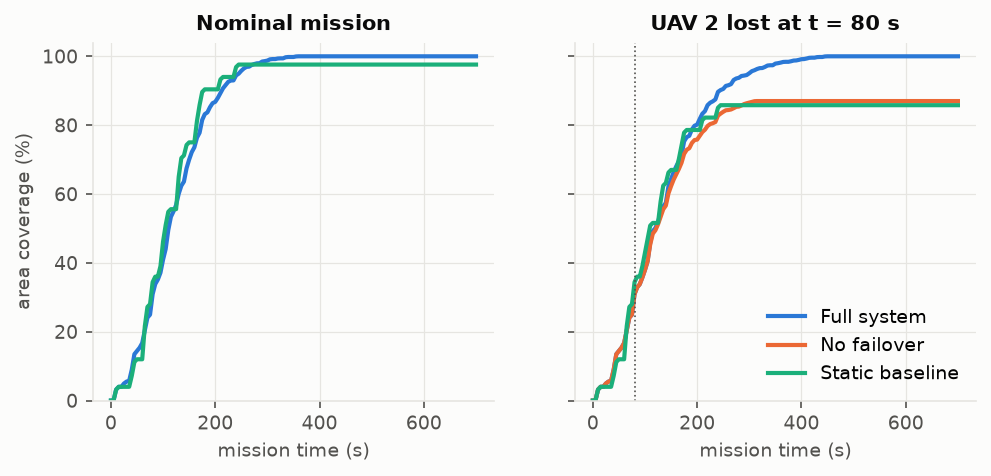
\includegraphics[width=0.36\textwidth]{coverage_over_time.png}\hfill
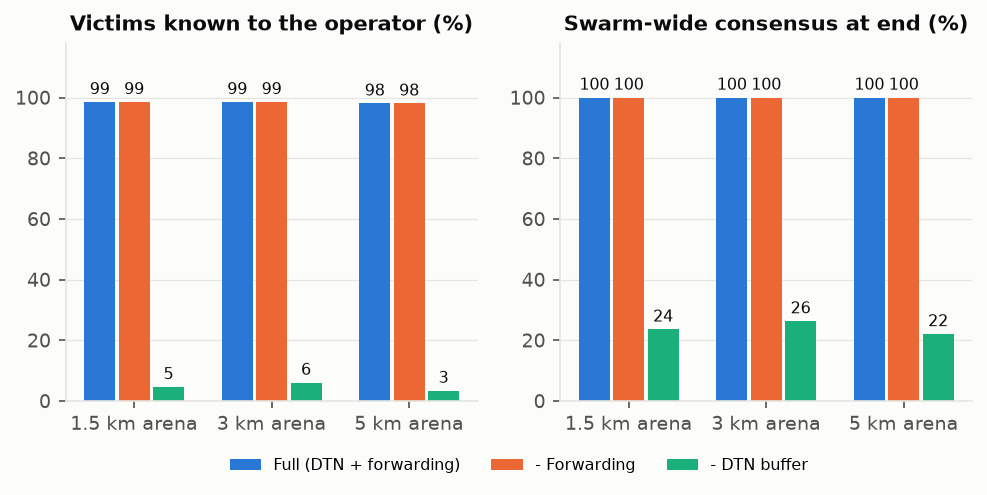
\includegraphics[width=0.36\textwidth]{network_ablation.png}
\caption{Left: coverage over time, nominal and with UAV~2 lost at 80\,s. Right: victims known to the operator, by arena size.}
\label{fig:covnet}
\end{figure*}

\begin{table*}[!t]
\caption{Forwarding policies (mean $\pm$ 95\% CI). Lat.: alert latency; Copies: per alert.}
\label{tab:dtn}
\centering\footnotesize
\setlength{\tabcolsep}{4pt}
\begin{tabular}{lrrrrrrrr}
\toprule
& \multicolumn{2}{c}{1.5\,km} & \multicolumn{2}{c}{3\,km} & \multicolumn{2}{c}{5\,km} & \multicolumn{2}{c}{3\,km, UAV lost}\\
\cmidrule(lr){2-3}\cmidrule(lr){4-5}\cmidrule(lr){6-7}\cmidrule(lr){8-9}
Policy & Lat.\,(s) & Copies & Lat.\,(s) & Copies & Lat.\,(s) & Copies & Lat.\,(s) & Copies\\
\midrule
Epidemic (proposed) & \textbf{34.3{\scriptsize$\pm$2.1}} & 4.12 & \textbf{41.0{\scriptsize$\pm$1.8}} & 4.30 & \textbf{102.9{\scriptsize$\pm$6.0}} & 3.39 & \textbf{46.3{\scriptsize$\pm$3.3}} & 3.52 \\
Spray-and-wait & 36.4{\scriptsize$\pm$2.5} & 2.38 & 48.6{\scriptsize$\pm$2.2} & 2.37 & 106.3{\scriptsize$\pm$5.3} & 2.14 & 56.4{\scriptsize$\pm$4.8} & 2.29 \\
Buffer only & 41.4{\scriptsize$\pm$2.3} & 1.00 & 59.2{\scriptsize$\pm$3.3} & 1.00 & 109.5{\scriptsize$\pm$5.7} & 1.00 & 66.4{\scriptsize$\pm$4.3} & 1.04 \\
\bottomrule
\end{tabular}

\end{table*}
\begin{figure*}[!t]
\centering
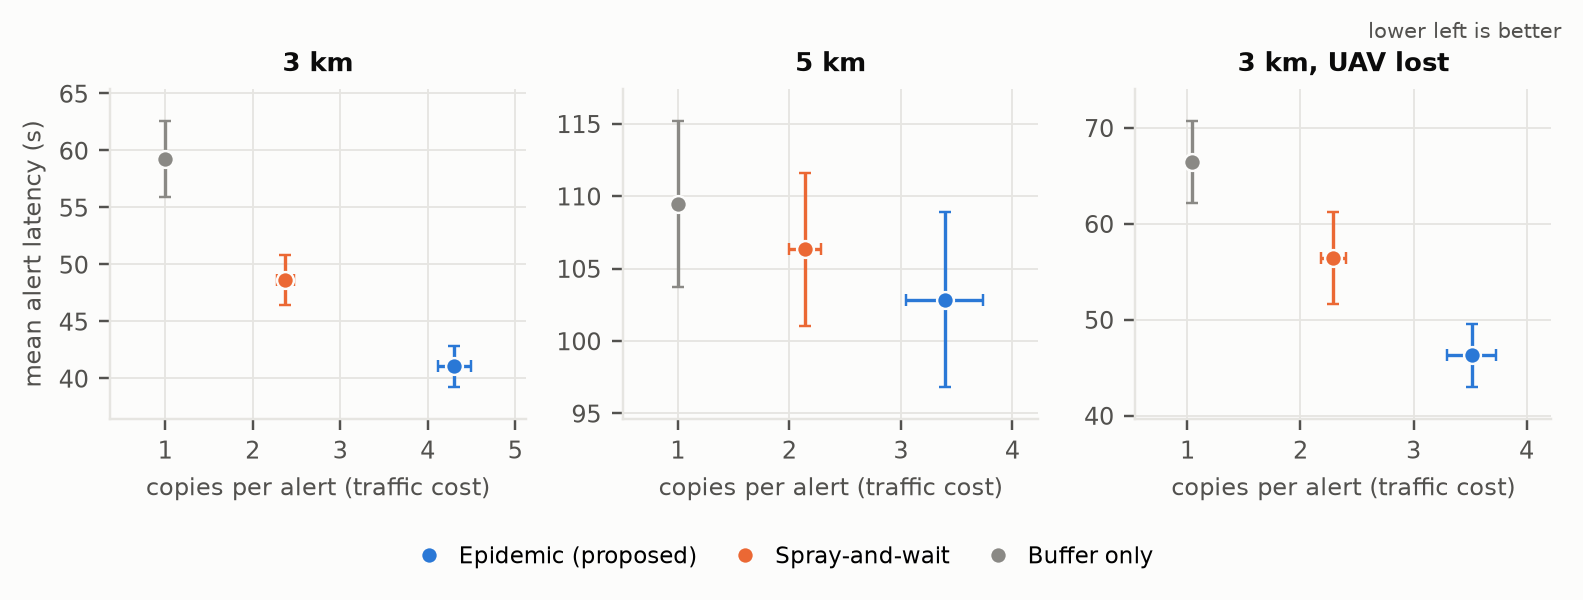
\includegraphics[width=0.5\textwidth]{forwarding_tradeoff.png}
\caption{Alert latency versus copies per alert (bars: 95\% CI).}
\label{fig:fwd}
\end{figure*}

\section{Results and Analysis}\label{sec:results}
\subsection{Detection Performance}
Table~\ref{tab:perc} shows that the fused model reaches an AP50 of 99.8 in daylight. Fusion is about 11 points better than thermal only, so the visible plane adds information, while removing it at night costs only 5.5 points because thermal carries most of the detection. Washout is the hardest case, because the network relies mainly on thermal: the recall falls to 0.39 while the precision stays at 0.99. The RGB-only case scores zero because the network was never trained without the thermal plane, so it says nothing about the value of RGB, and trained single-modality baselines are still needed (Section~\ref{sec:concl}).

Table~\ref{tab:speth} compares the daytime result with the base paper \cite{speth2022}, which reports YOLOv3 trained on the same dataset (Table~9 there, 485 aligned images with 891 people). Our fused YOLO11s model is ahead of their 4-channel model at AP50 (99.8 against 97.9) and at AP75 (85.8 against 76.9), and, like theirs, it is clearly ahead of the RGB-only and ensemble variants. The comparison is indicative only: we evaluate 150 of the 485 frames (275 people), the architecture (YOLO11s at 1280\,px against YOLOv3 at 960$\times$704) and schedule differ, so part of the gap comes from the newer detector and not from the fusion, AP50:95 was not computed, and the checkpoint was selected on the same split. Latencies are not comparable (CPU here, a drone-class GPU in \cite{speth2022}).





\subsection{Reference Mission Performance}
Without a failure, the decentralized swarm covers 100\% of the arena in \pmsd{353}{31}\,s (mean $\pm$ s.d.). Precision, recall and F1 are all \pmsd{0.980}{0.015}, where the whole-arena recall counts the victims in unsearched sectors. The mean localization error is \pmsd{1.45}{0.15}\,m, the first victim is detected after \pmsd{8.6}{7.2}\,s, and the operator learns of 100\% of the reports.


\begin{table*}[!t]
\caption{Allocation policies, nominal and with UAV~2 lost. Dup.: duplicate scans.}
\label{tab:alloc}
\centering\footnotesize
\setlength{\tabcolsep}{4pt}
\begin{tabular}{lrrrrrrrr}
\toprule
& \multicolumn{4}{c}{Nominal} & \multicolumn{4}{c}{UAV~2 lost}\\
\cmidrule(lr){2-5}\cmidrule(lr){6-9}
Policy & Cover.\,\% & Time (s) & Min.\,batt.\,\% & Dup. & Cover.\,\% & Time (s) & Min.\,batt.\,\% & Dup.\\
\midrule
EW-CVT (proposed) & \textbf{100.0} & 353 & \textbf{18.8} & \textbf{0.00} & \textbf{98.4} & 554 & 19.7 & 1.40 \\
Auction, no failover & \textbf{100.0} & \textbf{334} & 17.4 & 0.90 & 89.2 & \textbf{336} & 20.0 & 0.75 \\
Static partition & \textbf{100.0} & 364 & 17.9 & 0.10 & 87.6 & 353 & \textbf{20.3} & \textbf{0.30} \\
\bottomrule
\end{tabular}

\end{table*}
\begin{figure*}[!t]
\centering
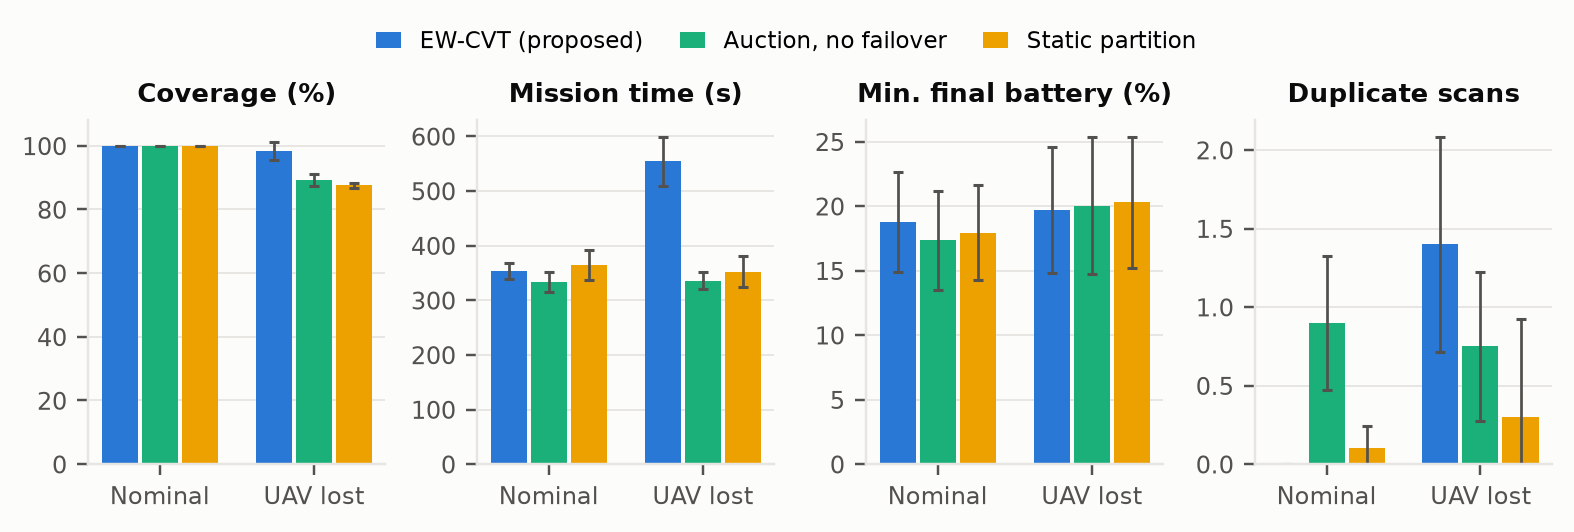
\includegraphics[width=0.5\textwidth]{allocation_baselines.png}
\caption{Allocation policies: coverage, time, battery and duplicates (bars: 95\% CI).}
\label{fig:alloc}
\end{figure*}

\subsection{Ablation Study}
Table~\ref{tab:abl} gives the effect of removing each component.


\emph{Failover} matters when a UAV is lost. The coverage after the loss is 98.4\% with failover and 87.4\% without it (Fig.~\ref{fig:covnet}, left), since without failover the sectors of the lost UAV are never searched.

\emph{Hysteresis} reduces churn but not flight time. In the full decentralized system it has almost no measurable effect, because the claims are already sticky (0.2 versus 0.4 sector flips). It matters when a global planner recomputes the partitions from fresh readings at every tick: hysteresis then cuts the commits about tenfold (296 to 31 per mission at $\sigma=2\%$) and the sector flips from 13.5 to 2.5, with the mission time unchanged.

\emph{EW weighting} is a trade-off. When $\alpha$ is swept from 0 to 3, the minimum final battery rises from 15.6\% to 20.3\% and the low-battery aborts fall from 0.95 to 0.30 per mission, but the mission becomes longer (377 to 488\,s) because the healthy UAVs carry more of the work.




\subsection{Comparison with Baseline Methods}\label{sec:base}
Table~\ref{tab:dtn} and Fig.~\ref{fig:fwd} compare the forwarding policies. Epidemic forwarding has the lowest alert latency in every scenario, but it also holds the most copies. At 3\,km, its latency is 7.6$\pm$1.7\,s below spray-and-wait (paired difference with 95\% confidence interval) and 18\,s below buffering only, and it keeps about 1.9 more copies per alert than spray-and-wait. When UAV~2 is lost, the operator recall is 0.978 with epidemic forwarding, 0.967 with spray-and-wait and 0.958 with buffering only, and the latency gap to spray-and-wait grows to about 10\,s. Otherwise the operator recall is the same for all policies.





Table~\ref{tab:alloc} and Fig.~\ref{fig:alloc} compare EW-CVT with a nearest-bidder auction without failover and with a static partition. Without a loss, all three reach full coverage. EW-CVT has no duplicate scans (0.00 against 0.90 and 0.10) and the highest minimum battery (18.8\% against 17.4\% and 17.9\%), but it is slower than the auction (353 against 334\,s). After a loss, the coverage is 98.4\% with failover against 89.2\% and 87.6\% for the auction and the static partition, and the arena recall is 0.96 against 0.87. The price is a longer mission, 554\,s against about 340\,s, because the survivors take over the work of the lost UAV. We credit the failover with the coverage gain.


\begin{table}[!t]
\caption{Recovery after the loss of UAV~2. Failover: time to the first claim of its sectors.}
\label{tab:dec}
\centering\footnotesize
\setlength{\tabcolsep}{3pt}
\begin{tabular}{lrrr}
\toprule
Scenario & Cover.\,\% & Time (s) & Failover (s)\\
\midrule
5\,km, no loss & 100.0 & 353 & n/a \\
5\,km, loss & 98.4 & 554 & 231 \\
3\,km, loss & 99.0 & 326 & 143 \\
1.5\,km, loss & 99.2 & 171 & 102 \\
\bottomrule
\end{tabular}

\end{table}

\subsection{Failure Recovery Analysis}
Table~\ref{tab:dec} shows the behaviour of the swarm when UAV~2 is lost. The survivors cannot know that the UAV is gone until it is overdue at base, so failover takes minutes. It takes 231\,s on average at 5\,km, 143\,s at 3\,km and 102\,s at 1.5\,km, and the shorter times in smaller arenas follow from the UAVs meeting more often. The coverage stays at 98.4\% or above, but the mission at 5\,km grows from 353\,s to 554\,s. In a few seeds, sectors stay unsearched because the survivors lack the battery for a second sortie.



\emph{Lease slack.} The slack trades detection speed against false alarms. For slack values of 20, 60, 120 and 240\,s, the mean failover latency is 192, 231, 293 and 411\,s, and the wrong suspicions fall from 11.2 of 15.6 to 0.4 of 4.7 per mission. Most suspicions concern UAVs that were fine (a landed UAV looks crashed to a peer in flight), but they cost little because released work is taken only at base. The status interval hardly affects the mission time (532 to 629\,s for 2 to 60\,s) until it approaches the duration of a contact.

%=====================================================================
\section{Discussion and Limitations}\label{sec:disc}
Our evidence clearly supports two conclusions: a sparsely connected swarm needs buffering, and losing a UAV costs coverage unless the others take over its work, with a delay set by how long the survivors need to learn of the loss. Hysteresis matters only where partitions are recomputed from noisy readings at every tick, and energy weighting buys reserve at the price of speed.

Several limitations apply. First, the simulator is kinematic, with constant speeds, linear battery drain and no wind, and the network results depend on the radio model. Second, each sector shows one static dataset frame, so the mission-level precision and recall mostly reflect the detector on these frames and the sectors that were visited. Third, the perception ablation masks one plane of a single fused network, and the training and validation frames come from the same site, so the absolute numbers are probably optimistic. Fourth, the decentralized design is simplified: the UAVs launch together and share the initial partition, status messages are single-hop, alerts are addressed to every UAV whether alive or not, and forwarding reads the holdings of the receiver instead of simulating the exchange on contact. The lease detector is one of several possible designs and has not been compared with the others, and the 15\% reserve and the noise levels are scenario assumptions.

%=====================================================================
\section{Conclusion and Future Work}\label{sec:concl}
This paper presented a decentralized search-and-rescue system for swarms that are mostly out of radio contact. It integrates early-fusion RGB and thermal perception, a delay-tolerant mesh with store-carry-forward relaying, and an energy-aware coordination layer without a central planner. Buffering was the largest effect that we measured. Failover recovers coverage after a UAV is lost, and epidemic relaying delivers alerts faster than spray-and-wait and buffering only, at the price of more copies. The price of decentralization is a failover latency of minutes. We have reported the unfavourable results and the limits of a simulation-only study.

Future work includes training separate RGB-only and thermal-only detectors for a proper modality ablation, comparing complete prior-work stacks across a sweep of network connectivity, letting status messages carry third-party state so that failure detection does not wait for an overdue return, and adding a camera model and richer wind and energy models.

%=====================================================================
\begingroup\scriptsize\setlength{\itemsep}{0pt}\setlength{\parskip}{0pt}\begin{thebibliography}{99}
\bibitem{hwang2015kaist} S.~Hwang, J.~Park, N.~Kim, Y.~Choi, and I.~S.~Kweon, ``Multispectral pedestrian detection: Benchmark dataset and baseline,'' in \emph{Proc. IEEE CVPR}, 2015.
\bibitem{liu2016multispectral} J.~Liu, S.~Zhang, S.~Wang, and D.~N.~Metaxas, ``Multispectral deep neural networks for pedestrian detection,'' in \emph{Proc. BMVC}, 2016.
\bibitem{zhang2019weakly} L.~Zhang \emph{et al.}, ``Weakly aligned cross-modal learning for multispectral pedestrian detection,'' in \emph{Proc. IEEE ICCV}, 2019.
\bibitem{redmon2016yolo} J.~Redmon, S.~Divvala, R.~Girshick, and A.~Farhadi, ``You only look once: Unified, real-time object detection,'' in \emph{Proc. IEEE CVPR}, 2016.
\bibitem{jocher2024yolo11} G.~Jocher and J.~Qiu, ``Ultralytics YOLO11,'' software, 2024. [Online]. Available: \nolinkurl{https://github.com/ultralytics/ultralytics}
\bibitem{speth2022} S.~Speth, A.~Gon\c{c}alves, B.~Rigault, S.~Suzuki, M.~Bouazizi, Y.~Matsuo, and H.~Prendinger, ``Deep learning with RGB and thermal images onboard a drone for monitoring operations,'' \emph{J. Field Robot.}, vol.~39, no.~6, pp.~840-868, 2022; dataset: \nolinkurl{https://www.nii-cu-multispectral.org}
\bibitem{lloyd1982} S.~P.~Lloyd, ``Least squares quantization in PCM,'' \emph{IEEE Trans. Inf. Theory}, vol.~28, no.~2, pp.~129-137, 1982.
\bibitem{du1999cvt} Q.~Du, V.~Faber, and M.~Gunzburger, ``Centroidal Voronoi tessellations: Applications and algorithms,'' \emph{SIAM Rev.}, vol.~41, no.~4, pp.~637-676, 1999.
\bibitem{cortes2004coverage} J.~Cort\'es, S.~Mart\'inez, T.~Karatas, and F.~Bullo, ``Coverage control for mobile sensing networks,'' \emph{IEEE Trans. Robot. Autom.}, vol.~20, no.~2, pp.~243-255, 2004.
\bibitem{cortes2005limited} J.~Cort\'es, S.~Mart\'inez, and F.~Bullo, ``Spatially-distributed coverage optimization and control with limited-range interactions,'' \emph{ESAIM Control Optim. Calc. Var.}, vol.~11, no.~4, pp.~691-719, 2005.
\bibitem{aurenhammer1987power} F.~Aurenhammer, ``Power diagrams: Properties, algorithms and applications,'' \emph{SIAM J. Comput.}, vol.~16, no.~1, pp.~78-96, 1987.
\bibitem{fall2003dtn} K.~Fall, ``A delay-tolerant network architecture for challenged internets,'' in \emph{Proc. ACM SIGCOMM}, 2003.
\bibitem{vahdat2000epidemic} A.~Vahdat and D.~Becker, ``Epidemic routing for partially connected ad hoc networks,'' Duke Univ., Tech. Rep. CS-2000-06, 2000.
\bibitem{spyropoulos2005spray} T.~Spyropoulos, K.~Psounis, and C.~S.~Raghavendra, ``Spray and wait: An efficient routing scheme for intermittently connected mobile networks,'' in \emph{Proc. ACM SIGCOMM WDTN}, 2005.
\bibitem{kosaka2023dmlt} K.~Kosaka, Y.~Noda, T.~Yokotani, and K.~Ishibashi, ``Implementation and evaluation of the control mechanism among distributed MQTT brokers,'' \emph{IEEE Access}, vol.~11, 2023, doi: 10.1109/ACCESS.2023.3335273.
\bibitem{baidya2018flynetsim} S.~Baidya, Z.~Shaikh, and M.~Levorato, ``FlyNetSim: An open source synchronized UAV network simulator based on ns-3 and Ardupilot,'' in \emph{Proc. ACM MSWiM}, 2018, pp.~37-45.
\bibitem{rappaport2002wireless} T.~S.~Rappaport, \emph{Wireless Communications: Principles and Practice}, 2nd~ed. Prentice Hall, 2002.
\bibitem{goodrich2008} M.~A.~Goodrich \emph{et al.}, ``Supporting wilderness search and rescue using a camera-equipped mini UAV,'' \emph{J. Field Robot.}, vol.~25, no.~1-2, pp.~89-110, 2008.
\bibitem{burgard2005} W.~Burgard, M.~Moors, C.~Stachniss, and F.~E.~Schneider, ``Coordinated multi-robot exploration,'' \emph{IEEE Trans. Robot.}, vol.~21, no.~3, pp.~376-386, 2005.
\bibitem{gerkey2004} B.~P.~Gerkey and M.~J.~Matari\'c, ``A formal analysis and taxonomy of task allocation in multi-robot systems,'' \emph{Int. J. Robot. Res.}, vol.~23, no.~9, pp.~939-954, 2004.
\bibitem{olfatisaber2007} R.~Olfati-Saber, J.~A.~Fax, and R.~M.~Murray, ``Consensus and cooperation in networked multi-agent systems,'' \emph{Proc. IEEE}, vol.~95, no.~1, pp.~215-233, 2007.
\bibitem{bekmezci2013} \.I.~Bekmezci, O.~K.~Sahingoz, and \c{S}.~Temel, ``Flying ad-hoc networks (FANETs): A survey,'' \emph{Ad Hoc Netw.}, vol.~11, no.~3, pp.~1254-1270, 2013.
\bibitem{zeng2016} Y.~Zeng, R.~Zhang, and T.~J.~Lim, ``Wireless communications with unmanned aerial vehicles: Opportunities and challenges,'' \emph{IEEE Commun. Mag.}, vol.~54, no.~5, pp.~36-42, 2016.
\bibitem{alhourani2014} A.~Al-Hourani, S.~Kandeepan, and S.~Lardner, ``Optimal LAP altitude for maximum coverage,'' \emph{IEEE Wireless Commun. Lett.}, vol.~3, no.~6, pp.~569-572, 2014.
\bibitem{jia2021llvip} X.~Jia, C.~Zhu, M.~Li, W.~Tang, and W.~Zhou, ``LLVIP: A visible-infrared paired dataset for low-light vision,'' in \emph{Proc. IEEE/CVF ICCV Workshops}, 2021.
\bibitem{wang2023yolov7} C.-Y.~Wang, A.~Bochkovskiy, and H.-Y.~M.~Liao, ``YOLOv7: Trainable bag-of-freebies sets new state-of-the-art for real-time object detectors,'' in \emph{Proc. IEEE/CVF CVPR}, 2023, pp.~7464-7475.
\bibitem{schwager2009} M.~Schwager, D.~Rus, and J.-J.~Slotine, ``Decentralized, adaptive coverage control for networked robots,'' \emph{Int. J. Robot. Res.}, vol.~28, no.~3, pp.~357-375, 2009.
\bibitem{demers1987} A.~Demers \emph{et al.}, ``Epidemic algorithms for replicated database maintenance,'' in \emph{Proc. ACM PODC}, 1987, pp.~1-12.
\bibitem{chandra1996} T.~D.~Chandra and S.~Toueg, ``Unreliable failure detectors for reliable distributed systems,'' \emph{J. ACM}, vol.~43, no.~2, pp.~225-267, 1996.
\bibitem{hayashibara2004} N.~Hayashibara, X.~D\'efago, R.~Yared, and T.~Katayama, ``The $\varphi$ accrual failure detector,'' in \emph{Proc. IEEE SRDS}, 2004, pp.~66-78.
\bibitem{gray1989} C.~G.~Gray and D.~R.~Cheriton, ``Leases: An efficient fault-tolerant mechanism for distributed file cache consistency,'' in \emph{Proc. ACM SOSP}, 1989, pp.~202-210.
\bibitem{kwok2007} A.~Kwok and S.~Mart\'inez, ``Energy-balancing cooperative strategies for sensor deployment,'' in \emph{Proc. IEEE CDC}, 2007, pp.~6136-6141.
\bibitem{munir2024} A.~Munir, A.~Dutta, and R.~Parasuraman, ``Energy-aware coverage planning for heterogeneous multi-robot system,'' arXiv:2411.02230, 2024.
\bibitem{grontved2023} K.~A.~R.~Gr{\o}ntved, U.~P.~S.~Lundquist, and A.~L.~Christensen, ``Decentralized multi-UAV trajectory task allocation in search and rescue applications,'' in \emph{Proc. IEEE ICAR}, 2023, pp.~35-41.
\bibitem{giacomossi2026} L.~Giacomossi \emph{et al.}, ``Market-based replanning for safety-critical UAV swarms in search and rescue missions,'' arXiv:2606.01970, 2026.
\end{thebibliography}\endgroup

\end{document}
